% book example for classicthesis.sty
\documentclass[
  % Replace twoside with oneside if you are printing your thesis on a single side
  % of the paper, or for viewing on screen.
  %oneside,
  twoside,
  %openleft,
  %titlepage,
  11pt, letterpaper,
  footinclude=true,
  headinclude=true,
  cleardoublepage=empty
]{book}

\usepackage{lipsum}
%\usepackage[linedheaders,parts,pdfspacing]{classicthesis}
\usepackage{amsmath}
\usepackage{amstext}
\usepackage{amsthm}
\usepackage{acronym}
\usepackage{cite} % para contraer referencias
\usepackage[utf8]{inputenc}
\usepackage[spanish]{babel}
\usepackage{graphicx}
\usepackage[bookmarks=true]{hyperref}
\usepackage{bookmark}
%\usepackage{pdfpages}
\usepackage{float}
\setlength{\parskip}{3mm}
\usepackage{marginnote}
\usepackage{url}


\title{ COMPUTACIÓN PERVASIVA APLICADA CREACIÓN ARTÍSTICA PARA LA RECONSTRUCCIÓN DE MEMORIA HISTÓRICA \\
Informe - Tesis de Maestría}

\author{Ing. Julian Olarte Ramos}

\begin{document}

\maketitle

\graphicspath{{images/}}

%*******************************************************
% Abstract
%*******************************************************
\pdfbookmark[1]{Abstract}{Abstract}
\chapter*{Resumen}

La reconstrucción de memoria histórica es uno de los principales mecanismos para la comprender las razones del origen y transformación del conflicto armado interno colombiano, sus diferentes actores y las vivencias de las víctimas que han sufrido de supresión y silenciamento. Uno de los mecanismos para reconstruir y procesar elementos de la memoria histórica del conflicto armado y comprender su magnitud es el arte y como objeto de estudio de éste trabajo, las instalaciones artísticas/interactivas que pudieran ser construidas con elementos de cómputo específicos en una combinación de arte digital. La computación pervasiva\footnote{Se propone el anglicismo \textit{'Computación Pervasiva'} que proviene de la frase \textit{'Pervasive Computation'} como descripción de la tecnología que será aplicada en éste trabajo de grado. Las traducciones de la palabra  \textit{pervasive} al español no proporcionan una acepción correcta de su significado en ingles y podrían distraer al lector de su significado original.}, describe un paradigma en las ciencias de la computación que investiga la creación de ambientes saturados de cómputo invisible, en el que las interfaces humano-máquina se extienden a muchos tipos de sensores y pueden responder a necesidades humanas basándose en espacios inteligentes, movilidad, computo distribuido, invisibilidad, escalabilidad local y respuesta a eventos heterogéneos. Este trabajo propone el montaje de una instalación interactiva como caso de estudio de aplicación de la computación pervasiva, teniendo como tema principal la reconstrucción de memoria histórica y la desaparición forzada; analizando su impacto, áreas de trabajo, proceso de construcción, proceso creativo, articulación con otras áreas de la ingeniería y de las ciencias humanas, y otras facetas que permitan su aprovechamiento, distribución y producción. 

%%*******************************************************
% Dedication
%*******************************************************
\thispagestyle{empty}
\pdfbookmark[1]{Dedication}{Dedication}

\vspace*{3cm}

\begin{center}
    A todos aquellos que se alejan de lo que más quieren para poder apreciarlo desde la distancia.   
\end{center}

%%*******************************************************
% Acknowledgments
%*******************************************************
\pdfbookmark[1]{Acknowledgements}{acknowledgements}
\chapter*{Agradecimientos}

Se agradece infinitamente a todos aquellos que aporten a ésta propuesta con sus críticas, ideas, elementos materiales o grandemente con la energía que pueda entregar. 
%*******************************************************
% Table of Contents
%*******************************************************
\pdfbookmark[1]{\contentsname}{tableofcontents}

\setcounter{tocdepth}{2} % <-- 2 includes up to subsections in the ToC
\setcounter{secnumdepth}{3} % <-- 3 numbers up to subsubsections

\tableofcontents

%*******************************************************
% List of Figures and of the Tables
%*******************************************************

%*******************************************************
% List of Figures
%*******************************************************    
\pdfbookmark[1]{\listfigurename}{lof}
\listoffigures

%*******************************************************
% List of Tables
%*******************************************************
%\pdfbookmark[1]{\listtablename}{lot}
%\listoftables
  
%*******************************************************
% List of Listings
%******************************************************* 
%\pdfbookmark[1]{\lstlistlistingname}{lol}
%\lstlistoflistings 
   
%*******************************************************
% Acronyms
%*******************************************************
%\pdfbookmark[1]{Acronyms}{acronyms}
%\chapter*{Acronyms}
%\begin{acronym}[UML]
%    \acro{DRY}{Don't Repeat Yourself}
%    \acro{API}{Application Programming Interface}
%    \acro{UML}{Unified Modeling Language}
%\end{acronym} 


\part{Definición}
%*******************************************************
% Capitulo uno
%*******************************************************

\chapter{Introducción}

Este trabajo propone el montaje de una instalación interactiva como caso de estudio en la aplcación del paradigma de Computación Pervasiva\cite{RN1}, analizando diferentes elementos como impacto, áreas de trabajo, proceso de construcción, proceso creativo, articulación con otras áreas de ingeniería y otras facetas que permitan su aprovechamiento como una tecnología útil en espacios artísticos. Como tema de estudio principal en la aplicación de la tecnología se usa la reconstrucción de memoria histórica del conflicto armado en Colombia y como eje principal, la magnitud del fenómeno de desaparición forzada. En este capítulo se describen brevemente los aspectos básicos del proyecto, sus objetivos, alcances y una comprensión básica del problema.    

\section{Presentación}

La reconstrucción de memoria histórica es uno de los principales mecanismos para la comprender las razones del origen y transformación del conflicto armado interno colombiano, sus diferentes actores y las vivencias de las víctimas que han sufrido de supresión y silenciamento. 

El Centro Nacional de Memoria Histórica (CNMH)\footnote{Centro Nacional de Memoria Histórica, http://www.centrodememoriahistorica.gov.co} es una institución adscrita al Departamento para la Prosperidad Social cuyo objetivo principal es contribuir a la realización de la reparación integral y el derecho a la verdad del que son titulares las víctimas. Bajo este objeto social se realizan actividades permanentes de construcción de memoria, destacando una gestión de iniciativas de memoria en las que el pueblo colombiano participa de forma permanente y autónoma. Al igual que esta institución muchas otras intituciones públicas e iniciativas privadas usan el arte como uno de los mecanismos para reconstruir y procesar elementos de la memoria histórica del conflicto armado. Uno de los referentes más importantes para este trabajo es el inventario de iniciativas artísticas gestionado por el CNMH. 

Como objeto de estudio de éste trabajo de grado se analizan las instalaciones interactivas que pudieran ser construidas con elementos de cómputo específicos en una combinación de arte plástico digital o interactivo. Existen numerosos ejemplos
\cite{RN35}\cite{RN25}\cite{RN34}\cite{RN38}\cite{RN31}\cite{RN29}\cite{RN40}\cite{RN37}
de creaciones digitales en las que el arte es el eje central y en las que la transformación del espacio a través de interfaces humano-máquina sale de esquemas tradicionales. También existen desde las artes liberales y las ciencias humanas investigaciones acerca de paz, guerra, memoria y arte, que permiten entender las diferentes aplicaciones del arte en temas de paz \cite{Jimenez201672}\cite{SotoAguilar201591}\cite{EstripeautBourjac2013154}. 

La computación pervasiva, describe una rama en las ciencias de la computación que investiga la creación de ambientes saturados de cómputo invisible, en el que las interfaces humano-máquina se extienden a muchos tipos de sensores. Según \cite{RN1}, la visión original de la computación pervasiva describe que los artefactos de un entorno serán fabricados de tal manera que los incrementos tecnológicos sean indistinguibles del objeto mismo. En este sentido el cómputo podrá impregnar de forma invisible la mayoría de objetos en un entorno y podrían recolectar información de forma transparente al usuario para después entregar respuestas en tiempo real o de forma natural.  Algunos de los retos y aspectos más importantes en la computación pervasiva son los espacios inteligentes, la movilidad, el computo distribuido, la invisibilidad, la escalabilidad local y la respuesta a eventos heterogéneos; todos aplicables al diseño de espacios artísticos con la ventaja de ser espacios que permiten una alta experimentación.

Como parte de este trabajo, se consultará y se recibirá apoyo de expertos en otras disciplinas fuera de la ingeniería de software, las interfaces humano-máquina y en general las ciencias de la computación; principalmente los temas de creación artística, instalaciones artísticas digitales, memorias del conflicto armado y desaparición forzada. Este trabajo cuenta con el apoyo del semillero de investigación en participación política y el consultorio de psicología, ambos del Politécnico Grancolombiano.

Bajo estos tres ejes principales y interdisciplinares: la computación pervasiva, la creación artística digital y la reconstrucción de memoria histórica; se presenta una propuesta de construcción de espacios de arte interactivo con un propósito social especifico del contexto del posconficto colombiano, que permite analizar la aplicabilidad de una tecnología que tiene el fin de transformar los espacios y los objetos con los que los humanos interactúan y en la que el entorno de aplicación en una situación que hace parte de la problemática y la situación actual de Colombia.


\section{Justificación}

La computación pervasiva incorpora diferentes áreas de conocimiento como interacción humano máquina, sistemas distribuidos, la computación móvil, los espacios inteligentes, la computación invisible; todas ellas con el fin de crear espacios en los que el cómputo permea el entorno humano de forma invisible e inteligente y en donde en el futuro los objetos y sus incrementos tecnológicos son indistinguibles. Investigaciones como [][][][] muestran casos de aplicación y frameworks que permiten comprender y experimentar la computación ubicua pero ninguna contempla el estudio desde la ingeniería de aplicaciones asociadas al arte digital. Por otro lado, publicaciones respecto de arte digital[][] presentan de una forma rica experiencias de construcción de instalaciones digitales pero su mirada no contempla tampoco el análisis desde el tema de computación ubicua. 

Además, la aplicación especifica de ésta tecnología sobre temas de reconstrucción de memoria es nula en cuanto a revisión bibliográfica. Por tanto, este trabajo pretende ampliar la base de investigación de la computación ubicua aplicada a áreas especificas de conocimiento, y en particular, al tema de reconstrucción de memoria del conflicto armado colombiano.   

\section{Objetivos}

\subsection{Objetivo principal}

Analizar las dinámicas de la aplicación de la computación pervasiva al diseño y montaje de una instalación artística sobre reconstrucción de memoria histórica y desaparición forzada.

\subsection{Objetivos específicos}

\begin{itemize}

    \item Recopilar información de contexto acerca de reconstrucción de memoria histórica y procesarla para incorporarla en un sistema de computo ubicuo.
    
    \item Analizar las metodologías de investigación-creación versus metodologías ágiles en la construcción de software para el propósito específico de éste trabajo de grado.

    \item Diseñar y construir un sistema software aplicando los conceptos de computación pervasiva.

    \item Realizar un montaje y presentación de la instalación artística junto con un análisis de su desempeño, funcionalidad, integración y usabilidad.

\end{itemize}

\section{Línea base cronograma}

\begin{enumerate}
	\item \label{puntouno} Recolección de información fuente acerca del conflicto armado colombiano a partir de la información del Centro de Memoria Histórica.
	\item \label{puntodos} Recolección de información de referentes y material audiovisual acerca de instalaciones artísticas que tengan componentes digitales.
	\item \label{puntotres} Procesamiento de la información de memoria histórica y su adaptación a sistemas ubicuos.
	\item \label{puntocuatro} Ciclos de diseño y desarrollo incrementales del software a usar en el montaje.
	\item \label{puntocinco} Montaje .
	
	
	
	
\end{enumerate}

\definecolor{midgray}{gray}{.5}
\begin{table}[!htbp]
	\centering
		\begin{tabular}{|c|c|c|c|c|c|c|c|c|c|c|}
		\hline
		&\multicolumn{5}{c|}{2010}&\multicolumn{5}{c|}{2010}\\
		\hline
		&MAR&ABR&MAI&JUN&JUL&AGO&SET&OUT&NOV&DEZ\\
		\hline
		\ref{ela-pro}&\cellcolor{midgray}&&&&&&&&&\\
		\hline
		\ref{anI}&&\cellcolor{midgray}&&&&&&&&\\
		\hline	
		\ref{anII}&&\cellcolor{midgray}&&&&&&&&\\
		\hline			
		\ref{anIII}&&\cellcolor{midgray}&\cellcolor{midgray}&&&&&&&\\
		\hline	
		\ref{dI}&&&\cellcolor{midgray}&&&&&&&\\
		\hline
		\ref{dII}&&&\cellcolor{midgray}&\cellcolor{midgray}&&&&&&\\
		\hline	
		\ref{dIII}&&&&\cellcolor{midgray}&\cellcolor{midgray}&&&&&\\
		\hline	
		\ref{esc-tcI}&&&\cellcolor{midgray}&\cellcolor{midgray}&\cellcolor{midgray}&&&&&\\
		\hline	
		\ref{imI}&&&&&\cellcolor{midgray}&&&&&\\
		\hline	
		\ref{imII}&&&&&&\cellcolor{midgray}&&&&\\
		\hline	
		\ref{imIII}&&&&&&\cellcolor{midgray}&\cellcolor{midgray}&\cellcolor{midgray}&&\\
		\hline	
		\ref{tec}&&&&&&&&\cellcolor{midgray}&\cellcolor{midgray}&\\
		\hline	
		\ref{esc-tcII}&&&&&&&&\cellcolor{midgray}&\cellcolor{midgray}&\cellcolor{midgray}\\
		\hline	
		\end{tabular}
\end{table}

\section{Alcance y entregables}

Éste proyecto se limitará a las siguientes:

\begin{itemize}
    \item Se realizará construcción y montaje de los diferentes elementos de la instalación artística desde las actividades del desarrollo de software y el diseño de sistemas ubicuos. No se contempla el estudio de construcción o diseño artístico, semiología, antropología o alguna otra disciplina fuera de la ingeniería, pero se analizará como esos diferentes elementos pueden ser relacionados con la computación ubicua.
    \item Se usará la información publicada por el centro de memoria histórica como referente principal. No se hará construcción o búsqueda de información de antecedentes históricos como parte de éste trabajo.
    \item No se realizarán estudios acerca de la dirección, escenografía, estética o actuación. Pero se analizará como esos diferentes elementos se pueden relacionar con la computación ubicua.
\end{itemize}

Al final de éste trabajo se espera:

\begin{itemize}
\item Información de reconstrucción de memoria histórica procesada de tal manera que pueda ser incorporada como parte de un sistema de computación ubicua en un espacio artístico. En éste proceso además es necesario encontrar mecanismos adecuados para representación de información bajo la filosofía de la tecnología propuesta.  
\item Los diseños y la construcción de un sistema software distribuido, móvil, invisible e inteligente para computo ubicuo para la instalación artística.
\item Un montaje y presentación de la instalación artística junto con el análisis del proceso y la experiencia. 
\end{itemize}

\section{Metodología}

El proceso de desarrollo del proyecto tiene tres etapas principales:
\begin{itemize}
    \item Recolección de referentes fundamentales y análisis de la información del conflicto armado colombiano. Esta fase deberá realizarse en acompañamiento de otras disciplinas. Además deberá realizarse un análisis de mecanismos de representación de la información escogida bajo la tecnología propuesta.
    
    \item Análisis, diseño y construcción de un sistema ubicuo para el problema propuesto. En esta fase solo habrá un desarrollador de software pero se utilizarán características de modelos de proceso iterativos e incrementales en coordinación con el diseño artístico.
    \item Montaje de la instalación artística. Este proceso incluye la caracterización del montaje y, posterior a la ejecución, documentación de la experiencia.
\end{itemize}


%*******************************************************
% Capitulo dos
%*******************************************************

\chapter{Marco teórico}

El Marco Teórico es el conocimiento mínimo necesario que se requiere para comprender el problema de investigación. La base teórica de referencia es la que permite comprender el problema y sus principales aspectos de detalle en toda su extensión. Las áreas principales que conciernen a ésta investigación son Interacción Humano-Máquina \cite{sigchi1992curricula}, Arquitectura Empresarial y Arquitectura de Software.

\section{Interacción Humano Máquina}

Según \cite{sigchi1992curricula} \footnote{Documento publicado en 1992 pero en su página web tiene fecha de actualización de 2009-07-29. http://old.sigchi.org/cdg/index.html} es una disciplina alrededor del diseño, evaluación e implementación de sistemas de computo interactivo para uso humano y el estudio de los fenómenos alrededor de esa interacción. 

Los problemas clásicos estudiados contemplan la interacción de los humanos en estaciones de trabajo utilizando dispositivos de entrada/salida tradicionales como pantallas y teclados. Los problemas actuales incluyen toda gama de dispositivos, tamaños de sistemas, medios de presentación, la ubicuidad y la transformación ambiental. 

En la literatura se encuentran numerosas referencias a la palabra \textit{machine} y su acepción cubre cualquier elemento de procesamiento donde se realice cómputo. Así, se puede analizar la interacción entre humanos y por ejemplo en dispositivos como datáfonos, tarjetas con chip, teléfonos celulares, tabletas, estaciones de trabajo tradicionales, electrodomésticos en el hogar hasta espacios inteligentes. El área de HCI (\textit{Human Computer Interaction}) es un área de estudio interdisciplinar de la ingeniería en donde las ciencias de la computación y el diseño industrial son muy importantes y transdisciplinar con áreas como la psicología, la sociología y la antropología. 

\subsection{Arquitectura de interfaces y Sistemas de computo}

Según \cite{sigchi1992curricula} uno de los elementos en los que se divide el estudio de HCI es la Arquitectura de interfaces y Sistemas de computo\footnote{Título de capítulo: \textit{Computer System and Interface Architecture}, Sec. 2.3.4. Unidad C. Pag 22. }, en la cual se pueden distinguir: dispositivos de entrada y salida, técnicas de interacción, tipos de interacción, gráficas por computador, arquitectura de la interacción.

\subsubsection{Dispositivos de entrada y salida}

Esta sub-área de conocimiento se encarga de los detalles técnicos de los dispositivos de entrada y salida entre humanos y máquinas. Los dispositivos de entrada son todos los posibles mecanismos por los cuales información que es generada por los humanos, de manera explicita o implícita, llega a los sistemas de cómputo. Algunos ejemplos pueden ser diferentes tipos de cámaras en combinación con mecanismos específicos (como seguimiento y reconocimiento del dedo índice o los ojos). De manera análoga, los mecanismos de salida incluyen todos los mecanismos de presentación de información visual, sonora o física. En los mecanismos de salida también se incluyen los actuadores sobre dispositivos hardware que no sean pantallas.

\subsubsection{Técnicas de interacción}

Este subconjunto del área de conocimiento describe todas las técnicas y arquitecturas básicas para la interacción con los humanos.

En interacciones de entrada podemos encontrar diferentes tipos de propósitos como seleccionar, especificar parámetros o controlar de manera continua alguna variable. Las técnicas sobre las entradas se pueden dividir en técnicas basadas en teclado, mouse, lápiz o voz. En interacciones de salida se pueden encontrar todos lo propósitos de salida, usualmente relacionados con transmitir, resumir, ilustrar o visualizar información. No descrito por el \textit{Curricula  for  human-computer  interaction} están también todas las formas de material multimedia y juegos en los cuales el componente multimedia es el más relevante. Las técnicas asociadas con la salida de información incluyen desplazamiento de pantalla, diagramación de ventanas, animaciones y proyecciones en espacios no tradicionales.

Output techniques (e.g., scrolling display, windows, animation, sprites, fish-eye displays)
Screen layout issues (e.g., focus, clutter, visual logic)
Dialogue Interaction Techniques:
Dialogue type and techniques (e.g., alphanumeric techniques, form filling, menu selection, icons and direct manipulation, generic functions, natural language)
Navigation and orientation in dialogues, error management
Multimedia and non-graphical dialogues: speech input, speech output, voice mail, video mail, active documents, videodisc, CD-ROM
Agents and AI techniques
Multi-person dialogues
Dialogue Issues:
Real-time response issues
Manual control theory
Supervisory control, automatic systems, embedded systems
Standards
"Look and feel," intellectual property protection
C3. Dialogue Genre {p. 24}

The conceptual uses to which the technical means are put. Such concepts arise in any media discipline (e.g., film, graphic design, etc.).

Interaction metaphors (e.g., tool metaphor, agent metaphor)
Content metaphors (e.g., desktop metaphor, paper document metaphor)
Persona, personality, point of view
Workspace models
Transition management (e.g., fades, pans)
Relevant techniques from other media (e.g., film, theater, graphic design)
Style and aesthetics
C4. Computer Graphics {p. 24}

Basic concepts from computer graphics that are especially useful to know for HCI.

Geometry in 2- and 3- space, linear transformations
Graphics primitives and attributes: bitmap and voxel representations, raster-op, 2-D primitives, text primitives, polygon representation, 3-D primitives, quadtrees and octtrees, device independent images, page definition languages
Solid modeling, splines, surface modeling, hidden surface removal, animation, rendering algorithms, lighting models
Color representation, color maps, color ranges of devices
C5. Dialogue Architecture {p. 25}

Software architectures and standards for user interfaces.

Layers model of the architecture of dialogues and windowing systems, dialogue system reference models
Screen imaging models (e.g., RasterOp, Postscript, Quickdraw)
Window manager models (e.g., Shared address-space, client-server), analysis of major window systems (e.g., X, New Wave, Windows, Open Look, Presentation Manager, Macintosh)
Models of application-to-dialogue manager connection
Models for specifying dialogues
Multi-user interface architectures "Look and feel"
Standardization and interoperability


\part{Desarrollo}
%*******************************************************
% Capitulo tres
%*******************************************************

\chapter{Caso de estudio}
\label{Caso_de_estudio}

Se propone la intervención artística 'No los olvidamos' como caso de estudio para este trabajo de grado. La intervención hace parte del trabajo del colectivo artístico \textit{'Aitawa: Reconstrucción de memoria histórica con arte'}. A continuación se describe el panorama general de la obra, sus participantes, los elementos digitales o interactivos que incorpora y su metodología de construcción.

\section{Antecedentes, propósito y resultados}

Como parte de su misión, entidades gubernamentales como la 'Unidad para las víctimas' o la secretaría de Gobierno con su 'Alta consejería para las víctimas', desarrollan procesos permanentes de reparación integral para las personas que fueron afectadas directamente por el conflicto armado colombiano para que ejerzan su ciudadanía y aporten a la consolidación de la paz. Como resultado de sus acciones se han realizado talleres en el pasado que permiten la reunión de diferentes grupos de víctimas y que éstos grupos creen vínculos sociales activos. Un grupo de éstas personas se ha reunido y ha creado un colectivo para desarrollar acciones artísticas que les permitan construir lazos entre ellos, hacer catarsis de las diferentes vivencias dentro del conflicto armado, hacer visibles muchas de sus inquietudes y necesidades, desarrollar medidas de reconstrucción simbólica y de memoria y además identificar entidades que apoyen su gestión.

Una de las acciones del colectivo fue el desarrollo de una intervención artística llamada 'No los olvidamos', la cual consistió en el desarrollo de varios talleres con población inscrita en el registro único de víctimas y en la que se desarrollaban diferentes temas acerca de la reconstrucción simbólica de la memoria de algunas de las vivencias de los participantes. El proceso se orientó principalmente al flagelo de desaparición forzada y contó con el apoyo del consultorio de psicología y del Semillero en participación política, ambos del Politécnico Grancolombiano.

Durante los talleres se realizaron pequeñas piezas de origami que los participantes usaban para representar algunas de sus memorias y se realizaban guias y talleres desarrollados por los miembros del Colectivo\footnote{Los talleres y las guías no hacen parte de éste trabajo de grado y son propiedad de sus respectivos autores.}. Algunos de los talleres incluyeron acciones que permitieron utilizar la metodolgía de construcción colectiva, la cual es una metodología usada para creación artística y cuyos resultados se usaron para la aplicación de la tecnología de computación pervasiva.

Todo el proceso fue acompañado por IDARTES\footnote{Instituto Distrital de las Artes - Idartes - http://www.idartes.gov.co} en el marco de participación ciudadana de construcción del Libro al Viento 2018, para el capítulo de poblaciones el cuál será escrito por Margarita García\cite{idartesmargarita}\footnote{Margarita García Robayo visita la capital con Bogotá Contada http://www.idartes.gov.co/es/noticias/margarita-garcia-robayo-visita-la-capital-con-bogota-contada} quién participó en el último taller que el colectivo realizó.

\begin{figure}[h]\label{togafarchimate}
\centering
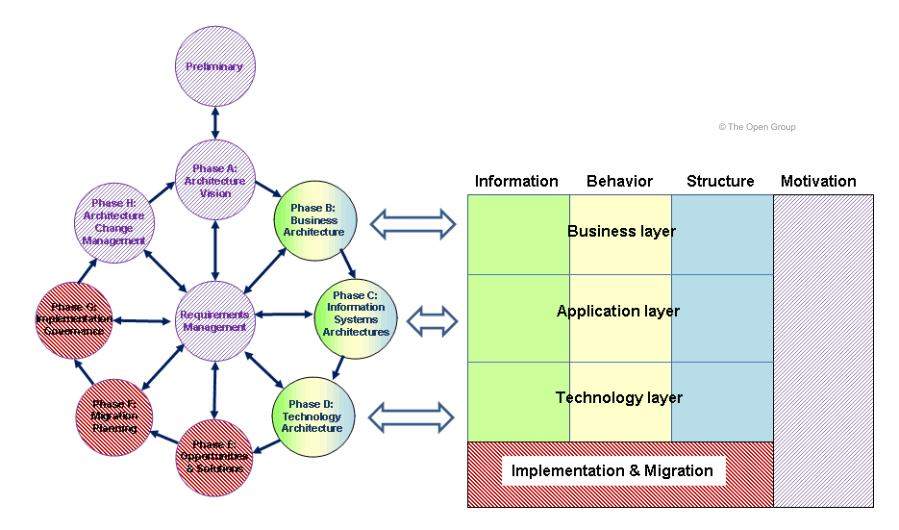
\includegraphics[scale=0.8]{togafarchimate}
\caption{Correspondencia entre Archimate y TOGAF.}
\end{figure}

\section{Talleres de construcción}

Entre las diferentes metodologías en creación de arte, el grupo decide que usará la \textit{creación colectiva}\cite{casacuberta2003creacion} y las analogías simbólicas\cite{garcia2003idea} como mecanismo para producir la obra. Numerosas obras de arte postmoderno son realizadas bajo este paradigma y en su caso las obras de arte quedan bajo la autoría de un autor principal y su grupo o bajo la autoría equilibrada de todo el grupo. Esta condición es supremamente importante en todas las decisiones que se toman frente a la aplicación de cualquier metodología de desarrollo de software. De este proceso se identifica durante el proceso realizado con los miembros del colectivo qué: 

\begin{itemize}
    \item Los requerimientos pueden cambiar ante cualquier idea que sea rápidamente aceptada por el grupo.
    \item Cada vez que los miembros del grupo desconocen uno de los elementos tecnológicos no avanzan hasta que lo comprenden del todo, incluso algunas veces no se alcanza su entendimiento.
    \item Se presenta iteraciones más numerosas en el diseño.
    \item El fin de los talleres de construcción puede ser otro al de diseñar la obra, por ejemplo describir memorias del pasado o crear piezas físicas para la obra final, por lo que se presenta confusión entre los participantes cuando se les habla de tecnología.
    \item Hay una clara distancia entre los participantes que no tienen ninguna formación técnica y el ingeniero, lo que provoca una brecha de vocabulario y comunicación.
\end{itemize}

\begin{figure}[h]\label{togafarchimate}
\centering
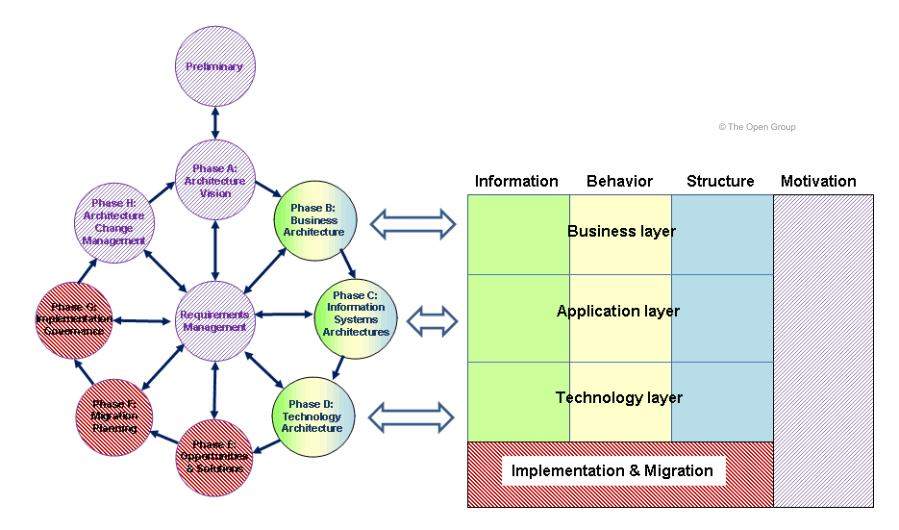
\includegraphics[scale=0.8]{togafarchimate}
\caption{Correspondencia entre Archimate y TOGAF.}
\end{figure}

Estas y otras consideraciones tiene un impacto altísimo en los modelos de proceso y las metodologías que deberían ser aplicadas en temas como este, disciplinas con las que se trabaja como ésta y en general en espacio no tradicionales de la ingeniería.  

\section{La obra}

El caso de estudio será desarrollado con la metodología de creación artística colectiva\cite{casacuberta2003creacion}. Todos los talleres desarrollados permitieron planear y construir una obra plástica digital e interactiva con la participación colectiva de los autores y los participantes de los talleres. La obra se propone como el taller final de la intervención artística y la cuál se incluye lo desarrollado en los talleres anteriores.

La presentación de la obra ocurre en el campus del Politécnico Grancolombiano en dos salones dispuestos para el evento: Uno de los salones para el desarrollo de taller y otro para la presentación de la instalación.

La obra consta de tres espacios y en dos de ellos hay elementos digitales. Tuvo un intervalo de dos horas de presentación y la coordinación, ensamble, desmontaje y convocatoria estuvo a cargo del autor de éste trabajo de grado.

\begin{figure}[h]\label{togafarchimate}
\centering
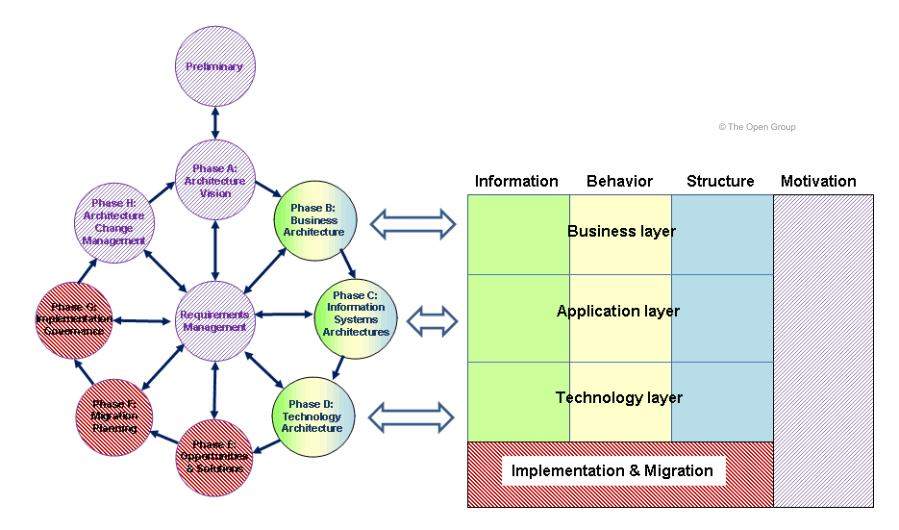
\includegraphics[scale=0.8]{togafarchimate}
\caption{Correspondencia entre Archimate y TOGAF.}
\end{figure}

\section{Los espacios}

La obra consta de tres espacios físicos: el primero de los espacios es llamado \textit{Presencia}, el segundo \textit{Ausencia} y el último \textit{Duelo}. El número tres es recurrente en la instalación y hace parte de su concepto de creación. A continuación se describen brevemente.

\begin{figure}[h]\label{togafarchimate}
\centering
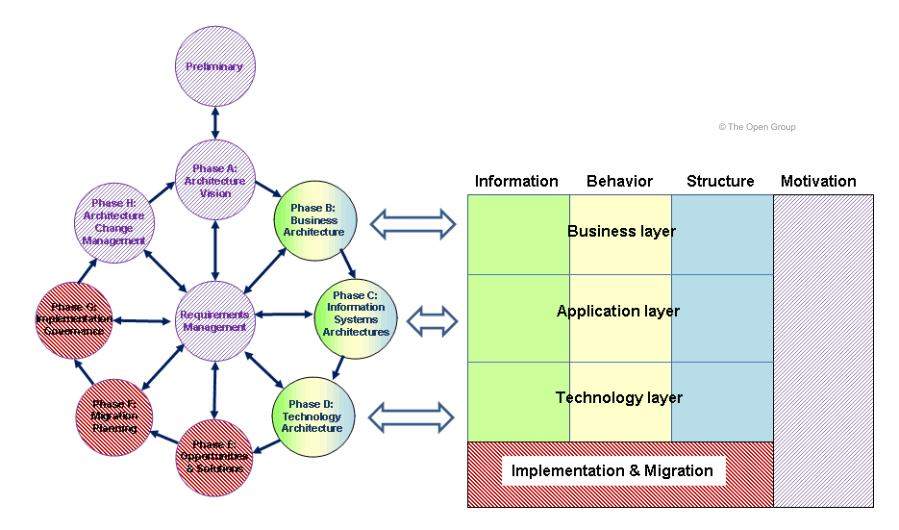
\includegraphics[scale=0.8]{togafarchimate}
\caption{Correspondencia entre Archimate y TOGAF.}
\end{figure}

\subsection{Presencia}

Es el inicio de la Instalación. El espacio consta de un mural de reconstrucción simbólica de la presencia de personas desaparecidas a partir de mariposas construidas en papel por los participantes de sesiones anteriores. En este espacio no hay ningún elemento de tecnología de forma deliverada. Tiene el objetivo de hacer contraste en la instalación y de representar la metáfora del inverso de la tecnología con la presencia humana. 

\begin{figure}[h]\label{togafarchimate}
\centering
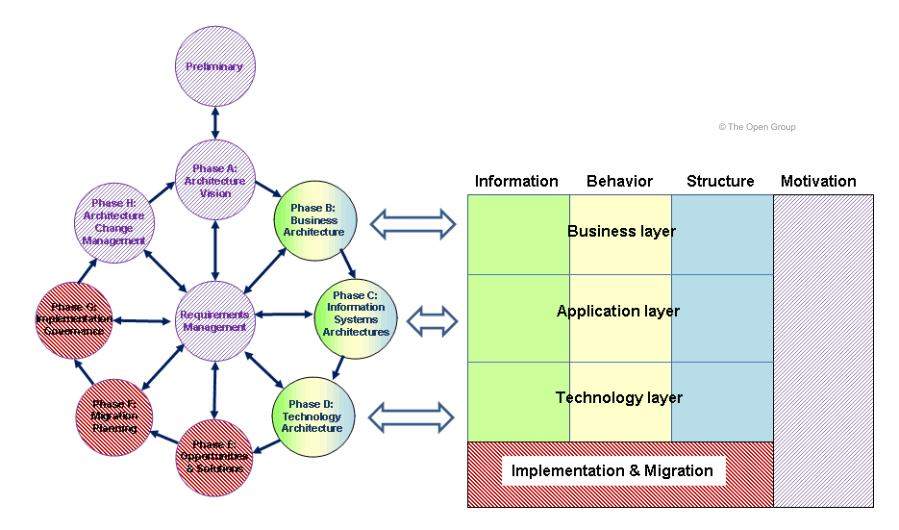
\includegraphics[scale=0.8]{togafarchimate}
\caption{Correspondencia entre Archimate y TOGAF.}
\end{figure}

\subsection{Ausencia}

Este espacio está caracterizado por una continuación del mural del primer espacio y por la presencia de objetos evocadores de memoria. Estos objetos fueron seleccionados en los talleres y componen la reconstrucción simbólica de situaciones vividas en algunos hechos violentos por los participantes. En este espacio hay tecnología de forma invisible: cuando los espectadores se acercan a los objetos se revelan imágenes en un televisor viejo dispuesto junto a los objetos. La selección de los elementos audiovisuales estuvo también a cargo de los participantes del colectivo. Este componente de tecnología es llamado el \textit{Espacio de memoria}.

\begin{figure}[h]\label{togafarchimate}
\centering
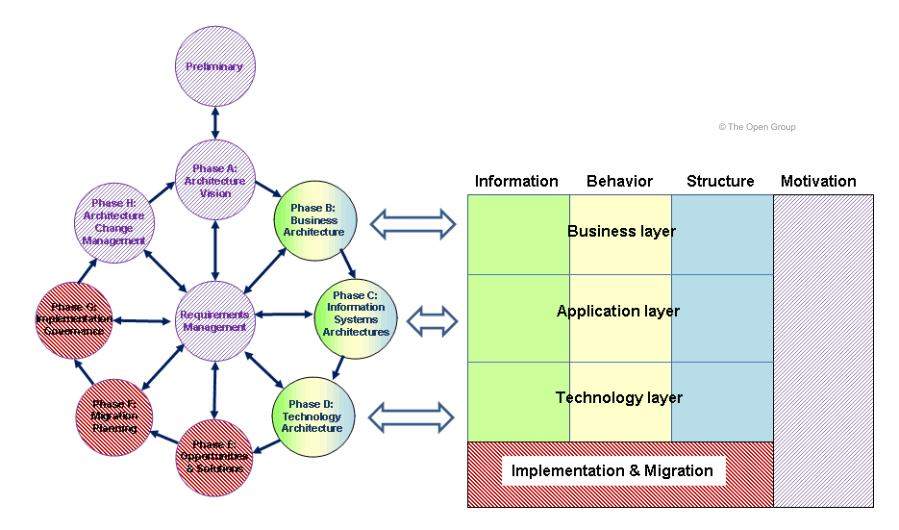
\includegraphics[scale=0.8]{togafarchimate}
\caption{Correspondencia entre Archimate y TOGAF.}
\end{figure}


\subsection{Duelo}

El último espacio representa el concepto de duelo continuado que tienen que padecer las víctimas del conflicto que sufren el fenómeno de desaparición forzada. El duelo continuado es la persistencia del estado de duelo cuando se desconoce si el desaparecido está vivo o muerto. Los familiares de desaparecidos viven en un constante estado de duelo durante el resto de su vida. Las consideraciones tecnológicas de este concepto psicológico no están contempladas como parte de este trabajo. En esta etapa hay varios elementos de tecnología que son bastante visibles y con los que se debe interactuar pero no son tradicionales: Un mural llamado \textit{El portal} se propone como componente de interacción táctil de espacio inteligente y con comunicación con el espacio anterior. Los contenidos mostrados en \textit{El portal} fueron creación del grupo y fueron desarrollados de forma colectiva.

\begin{figure}[h]\label{togafarchimate}
\centering
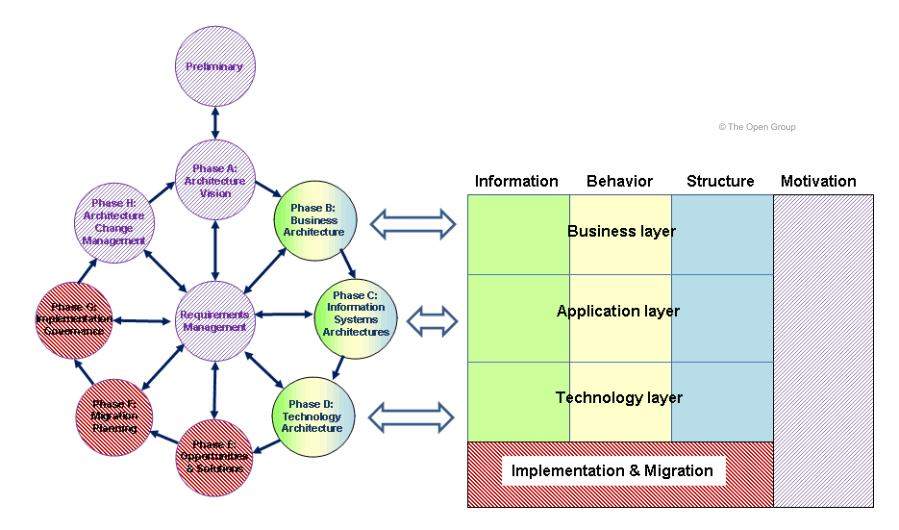
\includegraphics[scale=0.8]{togafarchimate}
\caption{Correspondencia entre Archimate y TOGAF.}
\end{figure}

\section{Componentes digitales}

Parte importante que debe ser descrita por este trabajo es el componente interactivo de la obra. El componente interactivo está representado en dos elementos ubicado en los dos últimos espacios; a saber, el primero llamado \textit{Espacio de memoria} y un segundo llamado \textit{El portal}, ambos descritos a continuación. 

\subsection{Espacio de memoria}

La reconstrucción de memoria tiene una metáfora recurrente en este espacio en donde se representan hechos vividos a través de objetos que guardan la evocación de experiencias del pasado. Cada objeto, escogido celosamente durante los talleres y el proceso de intervención, dispara una serie de recuerdos que solo la persona conoce en detalle y que hizo parte de su proceso de catarsis de las fatalidades del conflicto colombiano que tuvo que vivir.

En el espacio de memoria existe el concepto de invisibilidad de la tecnología\cite{RN13,weiser1991computer,RN23,RN14}, qué ha sido tratado por diversos autores en el contexto de computación pervasiva, en la que los humanos no se dan cuenta del computo o no se comunican de forma activa con las interfaces de usuario. Un visitante de la muestra simplemente interactuaría con los objetos y el televisor cambiaría de forma misteriosa de contenido multimedia. Es un concepto usado frecuentemente en museos y otras instalaciones interactivas, en \cite{RN31} por ejemplo, se explica  

\begin{figure}[h]\label{togafarchimate}
\centering
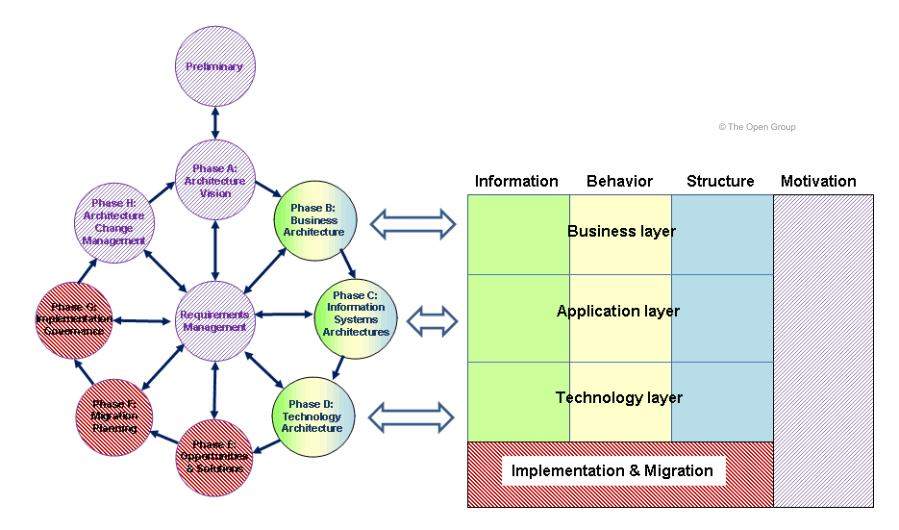
\includegraphics[scale=0.8]{togafarchimate}
\caption{Correspondencia entre Archimate y TOGAF.}
\end{figure}

\subsection{El Portal}

\begin{figure}[h]\label{togafarchimate}
\centering
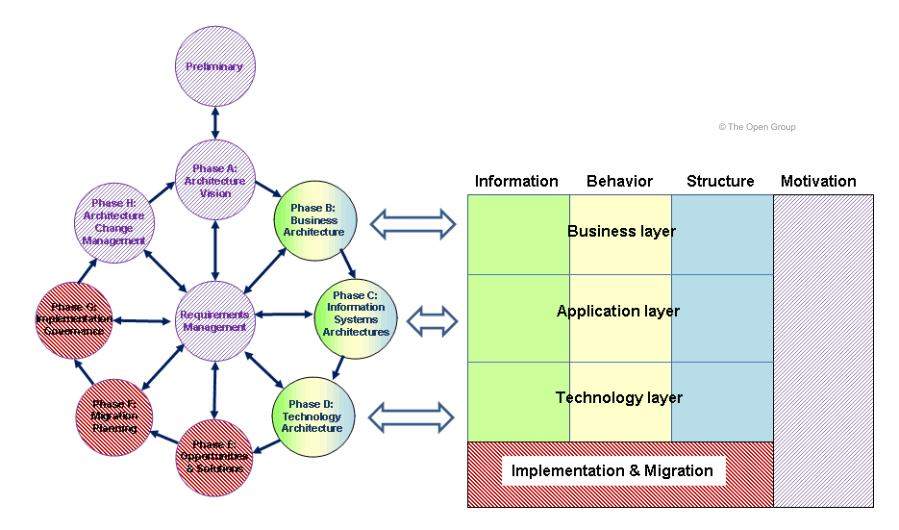
\includegraphics[scale=0.8]{togafarchimate}
\caption{Correspondencia entre Archimate y TOGAF.}
\end{figure}
%*******************************************************
% Capitulo cuatro
%*******************************************************

\chapter{Propuesta metodológica de producción}

\section{Potenciales metodologías de construcción de software}

Toma de decisiones acerca de la producción
Restricciones en la producción
Alcance tiempo costo en obras artísticas

\subsection{Metodologías duras}

\subsection{Metodologías ágiles}









\begin{figure}[h]\label{togafarchimate}
\centering
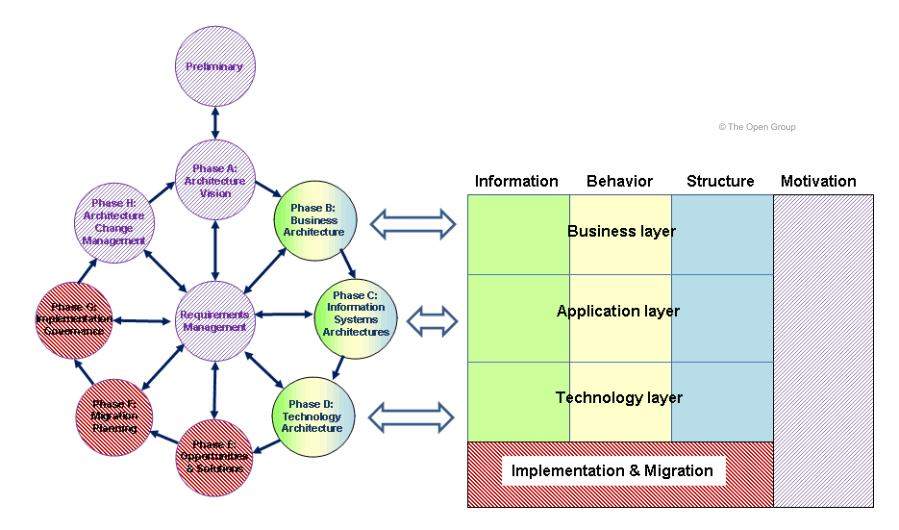
\includegraphics[scale=0.8]{togafarchimate}
\caption{Correspondencia entre Archimate y TOGAF.}
\end{figure}

%*******************************************************
% Capitulo cinco
%*******************************************************
\chapter{Diseño y construcción del software}

%%*******************************************************
% Capitulo seis
%*******************************************************

\chapter{Capa de negocio}

\marginpar{
    \begin{figure}[H]
        \includegraphics[scale=0.6]{IBusiness_actor}
    \end{figure} 
    \footnotesize 
    \textbf{Actor}. Una entidad organizacional que es capaz de ejecutar un comportamiento.
\newline
}
\marginpar{
    \begin{figure}[H]
        \includegraphics[scale=0.6]{IBusiness_role}
    \end{figure} 
    \footnotesize 
    \textbf{Rol}. La responsabilidad de llevar a cabo un comportamiento específico, al que se le puede asignar un actor.
\newline    
}
\marginpar{
    \begin{figure}[H]
        \includegraphics[scale=0.6]{IBusiness_collaboration}
    \end{figure} 
    \footnotesize 
    \textbf{Colaboración}.Un agregado de dos o más funciones de negocios que trabajan en conjunto para llevar a cabo un comportamiento colectivo.
}

\section{Organización}

El punto de vista de organización se centra en la organización de una empresa, un departamento, una red de empresas o cualquier otra entidad organizativa. Es posible presentar los modelos de este punto de vista como diagramas de bloques anidados o de una manera mas tradicional a través de un organigrama. Este punto de vista es muy útil en la identificación de las competencias, la autoridad y las responsabilidades dentro de la organización. 


\begin{figure}[h]
\centering
\includegraphics{organizacion}
\caption{Metamodelo del punto de vista organización.}
\end{figure}

En función del cumplimiento de los objetivos planteados, se propone la siguiente estructura organizacional para desarrollar el negocio.

\begin{figure}[h]
\centering
\includegraphics{Morganizacion}
\caption{Punto de vista organización.}
\end{figure}
 
\section{Cooperación de actor}

\marginpar{
    \begin{figure}[H]
        \includegraphics[scale=0.6]{ibusiness_interfaz}
    \end{figure} 
    \footnotesize 
    \textbf{Interfaz}.Un punto de acceso donde se pone a disposición un servicio de negocio para el entorno.
\newline
}
\marginpar{
    \begin{figure}[H]
        \includegraphics[scale=0.6]{ilocacion}
    \end{figure} 
    \footnotesize 
    \textbf{Ubicación}. Un lugar conceptual en el espacio.
\newline    
}


El punto de vista de cooperación de actor se centra en las relaciones de los actores entre sí y con su entorno. Un ejemplo común de esto es el "diagrama de contexto", lo que pone una organización con su entorno, que consiste en las partes externas, tales como clientes, proveedores y otros socios comerciales.Es muy útil en la determinación de dependencias externas y colaboraciones y muestra la cadena de valor o de la red en el que opera el actor. 

Otro uso importante es mostrar cómo una serie de actores comerciales y/o componentes de la aplicación en conjunto cooperan para realizar un proceso de negocio. Por lo tanto, en este punto de vista,le puede aplicar tanto a los actores comerciales o funciones y a los componentes de la aplicación.

\begin{figure}[h]
\includegraphics[scale=0.7]{cooperacion}
\centering
\caption{Metamodelo del punto de vista de cooperación de Actor.}
\end{figure}

Los stakeholders clave mantienen una relación con la estructura organizacional que se puede observar en la figura \ref{mcooperacionactor}.

\begin{figure}[h] 
\includegraphics[scale=0.7]{Mcooperacionactor}
\centering
\caption{Punto de vista de cooperación de Actor.}
\label{mcooperacionactor}
\end{figure}

\section{Función de negocio}

\marginpar{
    \begin{figure}[H]
        \includegraphics[scale=0.6]{ibusiness_funcion}
    \end{figure} 
    \footnotesize 
    \textbf{Función}. Un elemento de comportamiento que agrupa comportamientos basado en un conjunto seleccionado de criterios (por lo general requiere recursos de la empresa y/o competencias).
\newline
}El punto de vista de funciones de negocios muestra las principales funciones de negocio de una organización y sus relaciones en términos de los flujos de información, el valor, y bienes entre ellos. Este punto de vista es empleado para representar los aspectos más estables de una empresa en términos de las actividades primarias que realiza, independientemente de los cambios de organización o desarrollos tecnológicos. Por lo tanto, la arquitectura función de negocio de las empresas que operan en el mismo mercado a menudo presentan grandes similitudes. De esta manera, el punto de vista de la función empresarial proporciona una visión de alto nivel en las operaciones generales de la empresa, y se puede utilizar para identificar las competencias necesarias, o para estructurar una organización de acuerdo a sus actividades principales. El metamodelo se puede observar en la Figura \ref{funcion_de_negocio}.

\begin{figure}[H]   
\centering
\includegraphics{funcion_de_negocio}
\caption{Metamodelo del punto de vista de función de negocio.}
\label{funcion_de_negocio}
\end{figure}

Como parte de las funciones principales con algunos interesados se tiene la compra de servicios de tecnología como ads de publicidad o servicios de cloud y mantener alto el relacionamiento con los clientes. Esta lista de posibilidades de relación se puede consultar en la descripción canvas del relacionamiento con el cliente.

\begin{figure}[H]   
\centering
\includegraphics{MFuncionnegocio}
\caption{Punto de vista de función de negocio.}
\label{MFuncionnegocio}
\end{figure}


\section{Proceso de Negocio}


\marginpar{
    \begin{figure}[H]
        \includegraphics[scale=0.6]{ibusiness_interaccion}
    \end{figure} 
    \footnotesize 
    \textbf{Interacción}.Un elemento de comportamiento que describe el comportamiento de una colaboración.
\newline    
}
El punto de vista de procesos de negocio se utiliza para mostrar una estructura de alto nivel y la composición de uno o más procesos de negocio. Al lado de los mismos procesos, este punto de vista contiene otros conceptos directamente relacionados, como:
\marginpar{
    \begin{figure}[H]
        \includegraphics[scale=0.6]{ibusiness_evento}
    \end{figure} 
    \footnotesize 
    \textbf{Evento}.Algo que sucede (interna o externa) e influye en el comportamiento.
    \\
}

\marginpar{
    \begin{figure}[H]
        \includegraphics[scale=0.6]{ibusiness_proceso}
    \end{figure} 
    \footnotesize 
    \textbf{Proceso}. Un elemento de comportamiento que agrupa comportamientos basado en un ordenamiento de actividades.
}
\begin{itemize}
        \item Los servicios que ofrece un proceso de negocio con el mundo exterior, que muestra cómo un proceso contribuye a la realización de productos de la compañía.
        \item La asignación de los procesos de negocio a los roles, lo que da una idea de las responsabilidades de los actores asociados.
        \item La información utilizada por el proceso de negocio. 
\end{itemize}
Cada uno de ellos puede ser considerado como un "sub -view" de la vista de procesos de negocio.

\begin{figure}[H]
\centering
\includegraphics[scale=0.7]{proceso_de_negocio}
\caption{Punto de vista de proceso de negocio.}
\end{figure}

Se plantea entonces para esta propuesta los procesos más importantes frente al uso de la aplicación sin que sean menos relevantes la gestión comercial, el consumo de servicios de tecnología, las actividades de relacionamiento u otras descritas por el canvas. Son las actividades que hacen del uso de la aplicación un factor diferencial en proceso de negocio.

\begin{figure}[H]
\centering
\includegraphics[scale=0.8]{MProcesonegocio}
\caption{Metamodelo del punto de vista de proceso de negocio.}
\end{figure}

\marginpar{
    \begin{figure}[H]
        \includegraphics[scale=0.6]{ibusiness_servicio}
    \end{figure} 
    \footnotesize 
    \textbf{Servicio}.Un servicio que satisface una necesidad para un cliente (interno o externo de la organización).
\newline
}
\marginpar{
    \begin{figure}[H]
        \includegraphics[scale=0.8]{ibusiness_objeto}
    \end{figure} 
    \footnotesize 
    \textbf{Objeto}.Un elemento pasivo que es relevante desde una perspectiva de negocio. 
\newline    
}


\section{Cooperación de proceso de negocio}
El punto de vista de cooperación de proceso de negocio se utiliza para mostrar las relaciones de uno o más procesos de negocio entre sí y/o con su entorno. Puede ser utilizado tanto para crear un diseño de alto nivel de los procesos de negocio dentro de su contexto y para proporcionar un gestor operativo responsable de uno o más de estos procesos con penetración en sus dependencias. Algunos aspectos importantes del proceso de cooperación empresarial son:
\begin{itemize}
        \item Los causales de la relación entre los principales procesos de negocio de la empresa.
        \item Mapeo de los procesos de negocio en las funciones de negocio. 
        \item La realización de los servicios por parte de los procesos de negocio.
        \item El uso de datos compartidos.
\end{itemize}
\marginpar{
    \begin{figure}[H]
        \includegraphics[scale=0.8]{irepresentacion}
    \end{figure} 
    \footnotesize 
    \textbf{Representación}. Una forma perceptible de empaquetado de la información de un objeto de negocio. 
}\marginpar{
    \begin{figure}[H]
        \includegraphics[scale=0.8]{isentido}
    \end{figure} 
    \footnotesize 
    \textbf{Significado}.El conocimiento o experiencia presente en un objeto de negocio o de su representación, dado un contexto particular.
\newline
}Cada uno de ellos puede ser considerado como un "sub -view" de la vista de la cooperación de procesos de negocio.

\begin{figure}[h]
\centering
\includegraphics[scale=0.7]{cooperacion_de_proceso_de_negocio}
\caption{Metamodelo del punto de vista de cooperación de proceso de negocio.}
\end{figure}

Los procesos principales al rededor de la aplicación tienen que ver con los eventos en los que se detecta una interacción con una marca y se intenta documentar el resultado de la interacción. Esta información se usa para hacer posteriores comparaciones más adelante y divulgar la información de la gestión. Las marcas deberían reaccionar ante situaciones de percepción negativa y mejorar su calidad.

\begin{figure}[H]
\centering
\includegraphics[scale=0.8]{Mcooperacionproceso}
\caption{Punto de vista de cooperación de proceso de negocio.}
\end{figure}

\section{Producto}

\marginpar{
    \begin{figure}[H]
        \includegraphics[scale=0.8]{ivalor}
    \end{figure} 
    \footnotesize 
    \textbf{Valor}.El valor relativo, utilidad o importancia de un servicio o producto. 
}\marginpar{
    \begin{figure}[H]
        \includegraphics[scale=0.8]{iproducto}
    \end{figure} 
    \footnotesize 
    \textbf{Producto}. Una colección coherente de los servicios, acompañada de un contrato/conjunto de acuerdos, que se ofrece a los clientes (internos o externos). 
\newline
}

El punto de vista del producto representa el valor que estos productos ofrecen a los clientes u otras partes externas involucradas y se muestra la composición de uno o más productos en términos de la constitución (aplicación empresarial o) los servicios, y el contrato(s) asociado u otros acuerdos. 

También puede ser utilizado para mostrar las interfaces (canales) a través de los cuales se ofrece este producto, y los eventos asociados con el producto. El punto de vista del producto se usa frecuentemente en el desarrollo de productos para diseñar un producto mediante la composición de los servicios existentes o mediante la identificación de nuevos servicios que deben ser creados para este producto, dado el valor que un cliente espera. Puede entonces servir como entrada para los arquitectos de procesos de negocios y otros que necesitan para diseñar los procesos y las unidades que realizan estos productos.

\begin{figure}[H]
\centering
\includegraphics[scale=0.7]{producto}
\caption{Metamodelo del punto de vista de producto.}
\end{figure}


\marginpar{
    \begin{figure}[H]
        \includegraphics[scale=0.8]{icontrato}
    \end{figure} 
    \footnotesize 
    \textbf{Contrato}.Una especificación formal o informal de acuerdo que especifica los derechos y obligaciones inherentes a un producto. 
}

El producto actual está caracterizado por dos formas de negocio que suplen las condiciones de valor presentadas con el modelo canvas. La primera la aplicación móvil para los usuarios en donde pueden desarrollar servicios específicos generando valor de compartir información y con el impacto de la mejora de la calidad entre las marcas.

\begin{figure}[H]
\centering
\includegraphics[scale=0.9]{Mproducto}
\caption{Punto de vista de producto.}
\end{figure}


%%*******************************************************
% Capitulo siete
%*******************************************************

\chapter{Capa de aplicación}

\marginpar{
    \begin{figure}[H]
        \includegraphics[scale=0.6]{IAplication_component}
    \end{figure} 
    \footnotesize 
    \textbf{Componente}.Una parte modular, desplegable, y reemplazable de un sistema de software que encapsula su comportamiento y los datos y expone estos a través de un conjunto de interfaces. 
\newline
}La capa de aplicación describe los componentes lógicos que integran la solución que sirve a los intereses de la organización. A continuación se describen los puntos de vista de la capa.

\section{Comportamiento de aplicación}
El punto de vista del comportamiento de aplicación describe el comportamiento interno de una solicitud; por ejemplo, como se da cuenta de uno o más servicios de aplicación. Este punto de vista es útil en el diseño del comportamiento principal de aplicaciones, o en la identificación de solapamiento funcional entre diferentes aplicaciones.

\begin{figure}[H]
\centering
\includegraphics[scale=0.7]{comportamiento_de_aplicacion}
\caption{Metamodelo del punto de vista de comportamiento de aplicación.}
\end{figure}

\marginpar{
    \begin{figure}[H]
        \includegraphics[scale=0.5]{IApplication_collaboration}
    \end{figure} 
    \footnotesize 
    \textbf{Colaboración}. Un agregado de dos o más componentes de aplicaciones que funcionan en conjunto para llevar a cabo un comportamiento colectivo.
\newline
}

Identificados los tres servicios principales, se describe una estructura de componentes que cumple las funciones de gestionar las calificaciones, comparar las marcas y gestionar comentarios específicos que complementan la calificación. Otros servicios no incluidos en el punto de vista pueden ser la gestión de la información de la marca por su dueño.

\begin{figure}[H]
\centering
\includegraphics[scale=0.7]{Mcomportamientoaplicacion}
\caption{Punto de vista de comportamiento de aplicación.}
\end{figure}

\section{Cooperación de aplicación}
\marginpar{
    \begin{figure}[H]
        \includegraphics[scale=0.6]{IApplication_interface}
    \end{figure} 
    \footnotesize 
    \textbf{Interfaces}. Un punto de acceso donde se pone a disposición un servicio de aplicaciones para un usuario u otro componente de la aplicación
\newline
}El punto de vista de Cooperación de aplicación describe las relaciones entre los componentes de las aplicaciones en función de los flujos de información entre ellos, o en términos de los servicios que ofrecen y su uso. Es usado con frecuencia para crear una visión general del entorno de aplicaciones de una organización; también se utiliza para expresar la cooperación o la orquestación (interna) de los servicios que en conjunto apoyan la ejecución de un proceso de negocio.

\begin{figure}[H]
\centering
\includegraphics[scale=0.8]{cooperacion_de_aplicacion}
\caption{Metamodelo del punto de vista de Cooperación de aplicación.}
\end{figure}


\marginpar{
    \begin{figure}[H]
        \includegraphics[scale=0.6]{IApplication_function}
    \end{figure} 
    \footnotesize 
    \textbf{Función}. Un elemento de comportamiento que grupos un comportamiento automático que puede ser realizado por un componente de aplicación.
}

En la cooperación de aplicaciones vale la pena destacar que las fuentes de datos para obtener información que permita valorar no solo provienen de las experiencias de usuario registradas en la aplicación sino también de la minería de datos desde redes sociales u otras aplicaciones.

\begin{figure}[H]
\centering
\includegraphics[scale=0.8]{Mcooperacionaplicacion}
\caption{Punto de vista de Cooperación de aplicación.}
\end{figure}


\section{Estructura de aplicación}
\marginpar{
    \begin{figure}[H]
        \includegraphics[scale=0.6]{IApplication_interaction}
    \end{figure} 
    \footnotesize 
    \textbf{Interacción}. es un elemento que describe el comportamiento de una colaboración de aplicación.
\newline
}El punto de vista estructura de la aplicación muestra la estructura de una o más aplicaciones o componentes. Este punto de vista es útil en el diseño o la comprensión de la estructura principal de aplicaciones o componentes y los datos asociados; por ejemplo, para romper la estructura del sistema en construcción, o para identificar los componentes de aplicaciones heredadas que son adecuados para la migración/integración.

\begin{figure}[H]
\centering
\includegraphics[scale=0.7]{estructura_de_aplicacion}
\caption{Metamodelo del punto de vista de Estructura de aplicación.}
\end{figure}

El modelo de componentes está descrito por la siguiente figura \ref{Mestructuraaplicacion}. Es de resaltar la propuesta de servicios REST expuestos desde el servidor de aplicaciones y consumo desde la aplicación móvil y desde una aplicación WEB de gestión de información de marca.

\begin{figure}[H]
\centering
\includegraphics[scale=0.7]{Mestructuraaplicacion}
\caption{Punto de vista de Estrutura de aplicación.}
\label{Mestructuraaplicacion}
\end{figure}


\section{Uso de aplicación}

\marginpar{
    \begin{figure}[H]
        \includegraphics[scale=0.8]{IData_object}
    \end{figure} 
    \footnotesize 
    \textbf{Objeto de datos}. Un elemento pasivo que permite un proceso automatizado.
}

El punto de vista de uso de la aplicación se describe cómo se utilizan las aplicaciones para soportar uno o más procesos de negocio, y la forma en que son utilizados por otras aplicaciones. Puede ser utilizado en el diseño de una aplicación mediante la identificación de los servicios que necesitan los procesos de negocio y otras aplicaciones, o en el diseño de procesos de negocio mediante la descripción de los servicios que están disponibles. Por otra parte, ya que identifica las dependencias de los procesos de negocio en las aplicaciones, puede ser útil a los gestores operativos responsables de estos procesos.

\begin{figure}[H]
\centering
\includegraphics{uso_de_aplicacion}
\caption{Metamodelo del punto de vista de uso de aplicación.}
\end{figure}

Los procesos más importantes de la aplicación son realizados por unos componentes clave: la calificación de marca, la comparación entre marcas y la descripción de eventos entre marcas.

\begin{figure}[H]
\centering
\includegraphics{Musoaplicacion}
\caption{Punto de vista de uso de aplicación.}
\end{figure}



%%*******************************************************
% Capitulo nueve
%*******************************************************

\chapter{Capa de Infraestructura}

\section{Infraestructura}

\marginpar{
    \begin{figure}[H]
        \includegraphics[scale=0.6]{Inode}
    \end{figure} 
    \footnotesize 
    \textbf{Nodo}. Un recurso computacional donde cualquier artefacto se pueden almacenar o desplegar para ejecutar.
\newline
}
\marginpar{
    \begin{figure}[H]
        \includegraphics[scale=0.6]{Idevice}
    \end{figure} 
    \footnotesize 
    \textbf{Dispositivo}. Un recurso de hardware sobre el cual los artefactos se pueden almacenar o desplegar para su ejecución.
\newline
}

\marginpar{
    \begin{figure}[H]
        \includegraphics[scale=0.8]{Inetwork}
    \end{figure} 
    \footnotesize 
    \textbf{Red}.Un medio de comunicación entre dos o mas dispositivos.
}El punto de vista de infraestructura contiene los elementos de la infraestructura de hardware y software de apoyo a la capa de aplicación, tales como dispositivos físicos, redes o software del sistema (por ejemplo, sistemas operativos, bases de datos y middleware).

\begin{figure}[H]
\centering
\includegraphics[scale=0.7]{infraestructura}
\caption{Metamodelo del punto de vista de infraestructura.}
\end{figure}

La propuesta actual establece un servicio escalable en cloud con un proveedor el cual esconderá los detalles del servicio. Este proceso de ocultación incluye el ámbito completo de servicio conectividad, desempeño, y todos los aspectos de operación de la infraestructura.

Se propone entonces un uso de infraestructura sin detalle pero orientado a ciertas tecnologías en particular, como se ve en la figura \ref{Minfraestructura}.

\begin{figure}[H]
\centering
\includegraphics[scale=0.7]{Minfraestructura}
\caption{Punto de vista de infraestructura.}
\label{Minfraestructura}
\end{figure}

\section{Uso de infraestructura}
El punto de vista de uso de infraestructura muestra cómo las aplicaciones son compatibles con la infraestructura de software y hardware: los servicios de infraestructura son entregados por los dispositivos; software y sistemas de redes soportan las aplicaciones. Este punto de vista desempeña un papel importante en el análisis de rendimiento y escalabilidad, puesto que refiere a la infraestructura física para el mundo lógico de aplicaciones. Es muy útil en la determinación de los requisitos de rendimiento y calidad de la infraestructura basada en las exigencias de las diferentes aplicaciones que lo utilizan.

\begin{figure}[H]
\centering
\includegraphics[scale=0.7]{uso_de_infraestructura}
\caption{Metamodelo del punto de vista de uso de infraestructura.}
\end{figure}


\marginpar{
    \begin{figure}[H]
        \includegraphics[scale=0.8]{Isystem_software}
    \end{figure} 
    \footnotesize 
    \textbf{Software}. Un entorno de software para tipos específicos de componentes y objetos que son desplegados en forma de artefactos.
\newline
}Los componentes principales de la aplicación estarán distribuidos entre los servicios cloud y el software desplegado en cada dispositivo móvil. Otros elementos no descritos por el punto de vista pueden ser el marketplace: espacio externo para el host de la aplicación antes de ser descargada y el cliente para gestión de información de la marca.

\begin{figure}[H]
\centering
\includegraphics[scale=0.7]{Musoinfraestructura}
\caption{Punto de vista de uso de infraestructura.}
\end{figure}


\marginpar{
    \begin{figure}[H]
        \includegraphics[scale=0.6]{Icommunication_path}
    \end{figure} 
    \footnotesize 
    \textbf{Ruta de comunicación}. Un enlace entre dos o más nodos, a través del cual estos pueden intercambiar datos.
\newline
}

\marginpar{
    \begin{figure}[H]
        \includegraphics[scale=0.6]{Iinfraestructure_interface}
    \end{figure} 
    \footnotesize 
    \textbf{Interfaz de infraestructura}. Un punto de acceso donde los servicios de infraestructura ofrecidos por un nodo puede ser accedidos por otros nodos y componentes de la aplicación.
}

\section{Despliegue e implementación}
El punto de vista de despliegue e implementación muestra cómo se realizan una o más aplicaciones en la infraestructura. Esto comprende el mapeo de aplicaciones (lógicas) y componentes Onto artefactos (físicas), tales como Enterprise Java Beans, y el mapeo de la información utilizada por estas aplicaciones y componentes sobre la infraestructura de almacenamiento subyacente; por ejemplo, bases de datos o tablas de otros archivos. El punto de vista de implementación juega un papel importante en el análisis de rendimiento y escalabilidad, puesto que refiere la infraestructura física para el mundo lógico de aplicaciones. En seguridad y análisis de riesgos, el punto de vista de implementación se utiliza para identificar, por ejemplo, las dependencias y los riesgos críticos. 

\begin{figure}[H]
\centering
\includegraphics{organizacion_e_implementacion}
\caption{Metamodelo del punto de vista de despliegue e implementación.}
\end{figure}


Es importante destacar que cuando los componentes sean desplegados se comunicarán mediante el protocolo HTTPs sobre el puerto estándar 443.

\begin{figure}[H]
\centering
\includegraphics{Mdespliegueimplementacion}
\caption{Punto de vista de despliegue e implementación.}
\end{figure}

\section{Estructura de información}

El punto de vista de estructura de información es comparable a los modelos tradicionales de información creados en el desarrollo de casi cualquier sistema de información. Se muestra la estructura de la información utilizada en la empresa o en un proceso de negocio específico o aplicación, en términos de tipos de datos o las estructuras de clase (orientado a objetos). \marginpar{
    \begin{figure}[H]
        \includegraphics[scale=0.8]{Iinfraestructure_function}
    \end{figure} 
    \footnotesize 
    \textbf{Función de infraestructura}. Un elemento de comportamiento que agrupa un comportamiento de infraestructura que puede ser ejecutado por un nodo.
}
\marginpar{
    \begin{figure}[H]
        \includegraphics[scale=0.8]{Iartifact}
    \end{figure} 
    \footnotesize 
    \textbf{Artefacto}. Una pieza física de datos que es usada o producida en un proceso de desarrollo de software, o por la implementación y operación de un sistema.
}
Además, puede mostrar cómo la información a nivel empresarial está representado a nivel de aplicación en la forma de las estructuras de datos utilizadas allí, y cómo éstas son entonces mapeadas sobre la infraestructura subyacente; por ejemplo, por medio de un esquema de base de datos.

\begin{figure}[H]
\centering
\includegraphics{estructura_de_informacion}
\caption{Metamodelo del punto de vista de estructura de información.}
\end{figure}
Los elementos principales que deben ser modelados son las marcas y sus valoraciones. Adicionalmente las valoraciones deben ser representadas como las calificaciones cuantitativas y las valoraciones en texto o comentarios.

\begin{figure}[H]
\centering
\includegraphics{Mestructurainformacion}
\caption{Punto de vista de estructura de información.}
\end{figure}

\section{Realización del servicio}

\marginpar{
    \begin{figure}[H]
        \includegraphics[scale=0.8]{Iinfraestructure_service}
    \end{figure} 
    \footnotesize 
    \textbf{Servicio de infraestructura}. Una unidad visible externa de funcionalidad proporcionada por uno o más nodos, expuesta a través de interfaces bien definidas, y significativa para el entorno.
\newline
}


El punto de vista de realización de servicio se utiliza para mostrar cómo uno o más servicios de negocio se realizan mediante los procesos subyacentes (y algunas veces por componentes de la aplicación). De esta manera, se forma el puente entre el punto de vista de los productos comerciales y de procesos de negocio. Proporciona una "vista desde el exterior" en uno o más procesos de negocio.

\begin{figure}[H]
\centering
\includegraphics[scale=0.7]{realizacion_del_servicio}
\caption{Metamodelo del punto de vista de realización del servicio.}
\end{figure}

La realización de servicio describe los datos principales que serán gestionados desde la infraestructura montada. En este caso los componentes de software modificarán los datos principales que están descritos en la siguiente figura.

\begin{figure}[H]
\centering
\includegraphics[scale=0.7]{Mrealizacionservicio}
\caption{Punto de vista de realización del servicio.}
\end{figure}

\section{Capas}
El punto de vista en capas dibuja capas y aspectos de una arquitectura empresarial en un diagrama. Hay dos categorías de capas, capas dedicadas y capas de servicio. Las capas son el resultado de la utilización de la relación \textit{agrupación} para una partición natural de todo el conjunto de objetos y las relaciones que pertenecen a un modelo. La infraestructura, la aplicación, el proceso y los actores/roles pertenecen a la primera categoría. El principio estructural detrás de un punto de vista totalmente en capas es que cada capa dedicada expone, por medio de la relación "realización", una capa de servicios, que son más adelante "utilizado por" la siguiente capa dedicada. Por lo tanto, podemos separar fácilmente la estructura interna y la organización de una capa dedicada por parte de su comportamiento observable externamente expresado como la capa de servicio que da cuenta de la capa dedicada. El orden, número, o la naturaleza de estas capas no son fijos, pero en general una (más o menos) de estratificación completa y natural de un modelo ArchiMate deben contener la sucesión de capas descritas. El objetivo principal del punto de vista en capas es proporcionar información general en un diagrama. Además, este punto de vista se puede utilizar como apoyo para el impacto de análisis del cambio y análisis de rendimiento o para la ampliación de la cartera de servicios.

Una descripción transversal para el proyecto es mostrada en la siguiente figura \ref{mcapas}.


\begin{figure}[h]
\centering
\includegraphics[scale=0.7]{Mcapas}
\caption{Punto de vista de capas.}
\label{mcapas}
\end{figure}

%capitulo adicional patrones
%%*******************************************************
% Capitulo patrones
%*******************************************************

\chapter{Patrones}

Los patrones de diseño entregan descripciones de problemas comunes y sus soluciones tal que puedan ser reutilizados por la comunidad cada vez que se presenta el mismo problema. Un patrón describe un problema, su contexto y un esquema de solución que puede ser aplicado como plantilla.

En este capitulo se da una breve introducción a los patrones y de la sección \ref{patrones} en adelante se describe el conjunto de patrones de diseño que pueden ser aplicados en la solución.

\section{Tipos de patrones}

Los \textit{patrones de diseño} entregan descripciones de problemas comunes y sus soluciones tal que puedan ser reutilizados por la comunidad cada vez que se presenta el mismo problema. Un patrón describe un problema, su contexto y un esquema de solución que puede ser aplicado como plantilla.

Los \textit{patrones arquitectónicos} describen problemas de diseño amplios que se resuelven con transformaciones de la estructura desde una vista global.

Los \textit{patrones de datos} describen problemas recurrentes orientados a los datos y las soluciones para modelar con atributos específicos esos conjuntos de datos.

Los \textit{patrones de componentes} (también conocidos como diseño) establecen soluciones acerca de la construcción de entidades al nivel de componentes y subsistemas, y sus relaciones e interfaces.

\section{Patrones o estilos arquitectónicos}

Los patrones arquitectónicos, o patrones de arquitectura, también llamados arquetipos o estilos arquitectónicos ofrecen soluciones a problemas de arquitectura de software en ingeniería de software. Un patrón arquitectónico expresa un esquema de organización estructural esencial para un sistema de software, que consta de subsistemas, sus responsabilidades e interrelaciones. Dan una descripción de los elementos y el tipo de relación que tienen junto con un conjunto de restricciones sobre cómo pueden ser usados. En comparación con los patrones de diseño, los patrones arquitectónicos tienen un nivel de abstracción mayor.

Aunque un patrón arquitectónico comunica una imagen de un sistema, no es una arquitectura como tal. Un patrón arquitectónico es más un concepto que captura elementos esenciales de una arquitectura de software. Muchas arquitecturas diferentes pueden implementar el mismo patrón y por lo tanto compartir las mismas características o el mismo estilo. 

Uno de los aspectos más importantes de los patrones arquitectónicos es que encarnan diferentes atributos de calidad. Por ejemplo, algunos patrones representan soluciones a problemas de rendimiento y otros pueden ser utilizados con éxito en sistemas de alta disponibilidad. A primeros de la fase de diseño, un arquitecto de software escoge qué patrones arquitectónicos mejor ofrecen las calidades deseadas para el sistema.

\section{Patrones creacionales} \label{patrones}

Corresponden a patrones de diseño software que solucionan problemas de creación de instancias. Permiten encapsular y abstraer esos procesos de creación garantizando el cumplimiento de algunos atributos de calidad. Los patrones en ésta lista son \textit{Abstract factory}, \textit{Builder}, \textit{Prototype}, \textit{Singleton}.

\subsection{Abstract factory}

Este patrón permite describir la creación de familias de objetos a través de fabricas especificadas únicamente para ello.  En éste caso la creación de diferentes comentarios personalizados para las marcas es un tema que se contempla para desarrollos futuros. Debe ser posible construir diferentes tipos de comentarios para diferentes compañías y marcas. 

\begin{figure}[H]
\centering
\includegraphics[scale=0.6]{Pabstractfactory}
\caption{Patrón Fábrica abstracta.}
\end{figure}

En la imagen se puede ver que hay tanto jerarquías de familias como jerarquías de fábricas. Los productos serán las diferentes configuraciones de nuevos comentarios para las marcas.  Por ejemplo, un nuevo producto podría contar con encuesta de satisfacción con una configuración de preguntas específica.

\subsection{Builder}

El patrón Builder permite la construcción automatizada de objetos complejos. Algunas de las configuraciones de marcas productos y sub-productos podría llegara a ser bastante confusa o elaborada. Se propone el uso de este patrón para construir configuraciones especiales de familias de productos con modelos de valoración independiente.  

\begin{figure}[H]
\centering
\includegraphics[scale=0.65]{Pbuilder}
\caption{Patrón Builder.}
\end{figure}

Este patrón permite a través de una clase director, que puede ser parte del cliente constructor, hacer la invocación del Builder específico (concreto) para una de las marcas específicas.   

\subsection{Prototype}

Aunque el patrón prototype es comúnmente aplicado a objetos de no son del modelo del dominio también es posible aplicarlo a los objetos de valoración compleja que sean compuestos. En el caso de los comentarios pueden tener secuencias anidadas que admitan una copia profunda.

\begin{figure}[H]
\centering
\includegraphics[scale=0.65]{Pprototype}
\caption{Patrón Pototype.}
\end{figure}

La relación de herencia también puede ser una relación de implementación de una interfaz o se puede heredar el comportamiento clone desde la clase object. 

\subsection{Singleton}

Algunos comportamientos necesarios para adminstrar el control de concurrencia y el escalamiento de la aplicación serán realizados con la clase una clase singleton que registre el comportamiento de los nuevos componentes. Cada vez que un nuevo componente sea agregado deberá existir una clase que representa el directorio de plugins registrados y ésta solo podrá tener una Instancia que será lanzada al inicio de la aplicación.

\begin{figure}[H]
\centering
\includegraphics[scale=1.0]{Psingleton}
\caption{Patrón Singleton.}
\end{figure}


\section{Patrones estructurales}

Los patrones de diseño estructurales están enfocados en la gestión de la forma en la que las clases y los objetos se combinan para dar lugar a estructuras más complejas. Al igual que en las otros tipos de patrones, podemos hablar de patrones estructurales asociados a clases (Adapter) y asociados a objetos (Bridge, Composite, Decorator, Facade, Flyweight, Proxy). Los primeros utilizan la herencia mientras que los segundos se basan en la composición. Los patrones estructurales asociados a objetos describen formas de componer los objetos para conseguir nuevas funcionalidades. La flexibilidad de la composición de estos objetos surge de la posibilidad de cambiar dicha composición en tiempo de ejecución, lo que es imposible con la composición estática tradicional de clases.

\subsection{Adapter}

El patrón Adapter convierte la interfaz de una clase en la que otra necesita, permitiendo que clases con interfaces incompatibles trabajen juntas.

Por lo tanto, el uso de este patrón estructural está indicado cuando se quiere usar una clase ya implementada y su interfaz no es similar con la necesitada o cuando se desea crear una clase reusable que coopere con clases no relacionadas o que tengan interfaces compatibles.

\begin{figure}[H]
\centering
\includegraphics[scale=0.9]{Padapter}
\caption{Patrón Adapter.}
\end{figure}

Se espera que en la construcción de la aplicación todos los servicios REST funcionen como adapters en combinación con fachadas para exponer la funcionalidad de tratar a las entidades como modelos transitorios.

\subsection{Composite}

El patrón Composite sirve para construir objetos que estén formados por tros objetos más simples, pero siempre similares entre sí, gracias a la composición recursiva. Por lo tanto, al tener todos estos objetos una misma interfaz, el Composite simplifica el tratamiento de los mismos.

El patrón composite es ampliamente usado en el tratamiento de interfaces de usuario en las que se necesita, por ejemplo, representar un conjunto de elementos de una interfaz gráfica. Algunos de estos elementos serán simples, mientras que otros serán más complejos y estarán formados por varios elementos simples. Por tanto, el comportamiento y/o la información que proporciona un elemento complejo está determinada por los elementos que lo componen.
Generalizando, nos encontraríamos frente a una situación en la que necesitaríamos representar jerarquías de objetos de tipo parte y compuestos en la que se quiere usar la misma interfaz en las partes y en los compuestos. El patrón Composite, lo que nos ofrece es crear una interfaz o clase abstracta que actúe como superclase de las clases concretas que representan las partes y los compuestos. Las clases que representan los compuestos pueden ser tratadas como partes, porque soportan la interfaz.

\begin{figure}[H]
\centering
\includegraphics[scale=1]{Pcomposite}
\caption{Patrón Component.}
\end{figure}

\subsection{Decorator}

El patrón decorador permite la tarea de añadir dinámicamente funcionalidades a un Objeto. De este modo, elimina de necesidad de crear clases que fuesen heredando de la primera, incorporando no sólo la nueva funcionalidad, sino también otras nuevas y asociarlas a ella.

A veces se desea adicionar responsabilidades a un objeto pero no a toda la clase. Las responsabilidades se pueden adicionar por medio de los mecanismos de Herencia, pero este mecanismo no es flexible porque la responsabilidad es adicionada estáticamente. La solución flexible es la de rodear el objeto con otro objeto que es el que adiciona la nueva responsabilidad. Este nuevo objeto es el Decorator.

Este ejemplo de diseño  es útil cuando:
\begin{itemize}
    \item Se quiere añadir o expander las funcionalidades de objetos de forma dinámica y transparente. Con éste se logra escalar las funcionalidades a nuevas plateas rapidamente.
 \item Necesitamos que ciertas responsabilidades de un objeto puedan ser retiradas de forma sencilla en un futuro.
 \item No es posible o no compensa realizar esta expansión de funcionalidades mediante herencia.
 \item Existe la necesidad de expandir dinámicamente la funcionalidad de un objeto y/o eliminar la funcionalidad extendida.
\end{itemize}

\begin{figure}[H]
\centering
\includegraphics[scale=0.9]{Pdecorator}
\caption{Patrón decorador.}
\end{figure}


\subsection{Facade}

Provee una interfaz unificada para un grupo de interfaces en un subsistema, de manera que esta funcione como una interfaz de alto nivel que hace al resto de las interfaces fácil de usar.

\begin{figure}[H]
\centering
\includegraphics[scale=1.0]{Pfacade}
\caption{Patrón fachada.}
\end{figure}

Todos los servicios REST que serán creados estarán bajo la implementación de Facade.

\subsection{Flyweight}

El patrón Flyweight (u objeto ligero) sirve para eliminar o reducir la redundancia cuando tenemos gran cantidad de objetos que contienen información idéntica, además de lograr un equilibrio entre flexibilidad y rendimiento (uso de recursos).

\begin{figure}[H]
\centering
\includegraphics[scale=0.7]{Pflyweight}
\caption{Patrón flyweight.}
\end{figure}

\subsection{Proxy}

La finalidad principal del patrón de diseño estructural Proxy, es proporcionar un representante o sustituto de otro objeto para controlar el acceso a éste. Esto lo hace según la motivación de retrasar el costo de crear e inicializar un objeto hasta que sea realmente necesario. Por lo tanto, es usado cuando se necesita una referencia a un objeto más flexible o sofisticado que una referencia. Por ejemplo, si que queremos construir una aplicación que usa muchos objetos visuales, lo ideal es que dichos objetos sólo se instanciaran cuando se vayan a utilizar, de tal forma que se ahorre carga en memoria y tiempo.

\begin{figure}[H]
\centering
\includegraphics[scale=0.8]{Pproxy}
\caption{Patrón proxy.}
\end{figure}

Lo mismo ocurre cuando en el modelo de administración de persistencia debemos instanciar objetos o mantener en cache algunos otros que no sean persistentes.

\section{Patrones de comportamiento}

Los patrones de diseño software de comportamiento son aquellos que están relacionados con algoritmos y con la asignación de responsabilidades a los objetos.
Describen no solamente patrones de objetos o de clases, sino que también engloban patrones de comunicación entre ellos. Al igual que los otros tipos de patrones, se pueden clasificar en función de que trabajen con clases (Template Method, Interpreter) u objetos (Chain of Responsability, Command, Iterator, Mediator, Memento, Observer, State, Strategy, Visitor).

La variación de la encapsulación es la base de muchos patrones de comportamiento. Cuando un aspecto de un programa cambia frecuentemente, estos patrones trabajan con un objeto que encapsula dicho aspecto, teniendo que definir por tanto, una clase abstracta que describe la encapsulación del objeto.

\subsection{Chain of responsability}

Es un patrón de comportamiento que evita acoplar el origen de una petición a su receptor dando a más de un objeto la posibilidad de responder a una petición. Para ello, se encadenan los receptores y pasa la petición a través de la cadena hasta que es procesada por algún objeto. Este patrón es utilizado a menudo en el contexto de las interfaces gráficas de usuario donde un objeto puede estar compuesto de varios objetos (que generalmente heredán de una super clase "vista").

\begin{figure}[H]
\centering
\includegraphics[scale=0.9]{Pchainresponsability}
\caption{Patrón cadena de responsabilidad.}
\end{figure}

En este caso existe una cadena de mensajes en los comentarios de la marca y una cadena de publicación que son una serie de personas que autorizan o no la publicación de diferentes comentarios.

\subsection{Command}

El patrón de diseño software de comportamiento Command permite realizar una operación sobre un objeto sin conocer realmente las instrucciones de esta operación ni el receptor real de la misma. Esto se consigue encapsulando la petición como si fuera un objeto, con lo que además se facilita la parametrización de los métodos.

\begin{figure}[H]
\centering
\includegraphics[scale=1.0]{Pcomando}
\caption{Patrón Comando.}
\end{figure}

\subsection{State}

En determinadas ocasiones, cuando el contexto en el que se está desarrollando requiere que un objeto tenga diferentes comportamientos según el estado en que se encuentra, resulta complicado poder manejar el cambio de comportamientos y los estados de dicho objeto, todos dentro del mismo bloque de código. El patrón State propone una solución a esta complicación, creando básicamente, un objeto por cada estado posible del objeto que lo llama. Permite a un objeto alterar su comportamiento según el estado interno en que se encuentre.

Existe una extrema complejidad en el código cuando se intenta administrar comportamientos diferentes según una cantidad de estados diferentes. Asimismo el mantenimiento de este código se torna difícil, e incluso se puede llegar en algunos casos puntuales a la incongruencia de estados actuales por la forma de implementación de los diferentes estados en el código (por ejemplo con variables para cada estado).

\begin{figure}[H]
\centering
\includegraphics[scale=1.0]{Pstate}
\caption{Patrón State.}
\end{figure}

\subsection{Strategy}

Este es un patrón de diseño software de comportamiento que determina la forma de implementar el intercambio de mensajes entre diferentes objetos que realizan diferentes tareas, pero que comparten elementos comunes. El patrón de comportamiento Strategy permite gestionar un conjunto de operaciones de entre los cuales el cliente puede elegir el que le convenga más en cada situación, e intercambiarlo, de forma dinámica, cuando lo necesite.

Para llevar a cabo esta funcionalidad, este patrón de comportamiento trabaja con los algoritmos que implementan las diferentes estrategias de forma que los encapsula en una jerarquía, consiguiendo que el cliente trabaje contra un objeto intermediario o 'Context'. En este punto, el cliente puede elegir el algoritmo que prefiera de entre los implementados en las estrategias del sistema, o dejar al contexto la tarea de elegir al más apropiado para cada situación concreta.
Por lo tanto, cualquier sistema que presente un servicio o función determinada, que pueda o deba ser realizada de varias maneras dependiendo del contexto, será indicado gestionarlo con el patrón Strategy.

\begin{figure}[H]
\centering
\includegraphics[scale=0.8]{Pstrategy}
\caption{Patrón Strategy.}
\end{figure}

\subsection{Interpreter}

El interpreter es un patrón de diseño que, dado un lenguaje, define una representación para su gramática junto con un intérprete del lenguaje.

Se usa para definir un lenguaje para representar expresiones regulares que representen cadenas a buscar dentro de otras cadenas. Además, en general, para definir un lenguaje que permita representar las distintas instancias de una familia de problemas.

Se requiere para hacer análisis gramatical en la aplicación y determinar palabras clave en los comentarios.

\begin{figure}[H]
\centering
\includegraphics[scale=0.8]{Pinterpreter}
\caption{Patrón Interprete.}
\end{figure}

\subsection{Iterator}

El patrón de diseño de comportamiento Iterator es uno de los mayores exponentes de los patrones de comportamient. Presenta la interfaz que declara los métodos necesarios para acceder, de forma secuencial, a los objetos de una colección.

El iterator cubre la necesidad de acceder a los elementos de un contenedor de objetos sin tener que trabajar con su estructura interna. Además, es posible que se necesite más de una forma de recorrer la estructura siendo para ello necesario crear modificaciones en la clase. Mediante el uso del patrón, se añaden métodos que permiten recorrerla sin referenciar su representación, por lo que la responsabilidad del recorrido se traslada a un objeto iterador.

La gran desventaja de que usar este objeto iterador, más o menos encapsulado, es que muchas veces se necesita conocer la estructura del contenedor para elegir del tipo de iterador más adecuado. Esto se soluciona abstrayendo los tipos de los distintos iteradores y dotando a las estructuras de un método que cree un iterador concreto.

\begin{figure}[H]
\centering
\includegraphics[scale=0.7]{Piterator}
\caption{Patrón Iterador.}
\end{figure}

\subsection{Mediator}

El patrón mediador define un objeto que encapsula cómo un conjunto de objetos interactúan. Este patrón de diseño está considerado como un patrón de comportamiento debido al hecho de que puede alterar el comportamiento del programa en ejecución.

Habitualmente un programa está compuesto de un número de clases (muchas veces elevado). La lógica y computación es distribuida entre esas clases. Sin embargo, cuantas más clases son desarrolladas en un programa, especialmente durante mantenimiento y/o refactorización, el problema de comunicación entre estas clases quizás llegue a ser más complejo. Esto hace que el programa sea más difícil de leer y mantener. Además, puede llegar a ser difícil cambiar el programa, ya que cualquier cambio podría afectar código en muchas otras clases.

Con el patrón mediador, la comunicación entre objetos es encapsulada con un objeto mediador. Los objetos no se comunican de forma directa entre ellos, en lugar de ello se comunican mediante el mediador. Esto reduce las dependencias entre los objetos en comunicación, reduciendo entonces la Dependencia de código.


\begin{figure}[H]
\centering
\includegraphics[scale=1]{Pmediator}
\caption{Patrón Mediador.}
\end{figure}

\subsection{TemplateMethod}

El método de template está diseñado para marcos, donde cada cual implementa las partes invariables de la arquitectura de un ámbito, dejando "placeholders" para personalizar las opciones. Esto es un ejemplo de inversión de control. Alguna razones por la que se utiliza el método de plantilla son:

Dejar que las subclases que se implementan (a través del método primordial) tengan un comportamiento que puede variar.

Evitar duplicación en el código: la estructura general de flujo de trabajo, está implementada una vez en el algoritmo de clase abstracta, y variaciones necesarias son implementadas en cada de las subclases.

Control en qué punto(s) la subclassing está permitida. En oposición a una sencilla sobrecarga polimórfica, donde el método de base sería enteramente reescrito, permitiendo un cambio radical en el flujo. Sólo los detalles específicos del flujo se pueden cambiar.

\begin{figure}[H]
\centering
\includegraphics[scale=0.8]{Ptemplatemethod}
\caption{Patrón Template Method.}
\end{figure}

\subsection{Memento}

Memento es un patrón cuya finalidad es almacenar el estado de un objeto (o del sistema completo) en un momento dado de manera que se pueda restaurar en ese punto de manera sencilla, además sirve para facilitar a la gente floja realizar los programas. Para ello se mantiene almacenado el estado del objeto para un instante de tiempo en una clase independiente de aquella a la que pertenece el objeto (pero sin romper la encapsulación), de forma que ese recuerdo permita que el objeto sea modificado y pueda volver a su estado anterior. Aunque suele ser poco pertinente para su uso.

\begin{figure}[H]
\centering
\includegraphics[scale=0.9]{Pmemento}
\caption{Patrón Memento.}
\end{figure}

\subsection{Observer}

El patrón de comportamiento Observer define una interacción entre objetos, de manera que cuando uno de ellos cambia su estado, el Observer se encarga de notificar este cambio a los demás.

Por tanto, la razón de ser de este patrón es desacoplar las clases de los objetos, aumentando la modularidad del lenguaje y evitando bucles de actualización.

La idea básica del patrón es que el objeto de datos (o sujeto) contenga atributos mediante los cuales cualquier objeto observador (o vista) se pueda suscribir a él pasándole una referencia a sí mismo. De este modo, el sujeto mantiene así una lista de las referencias a sus observadores.

Dadas estas propiedades, el patrón Observer suele emplearse en el desarrollo de frameworks de interfaces gráficas orientados a objetos, enlazando 'listeners' a los objetos que pueden disparar eventos.

\begin{figure}[H]
\centering
\includegraphics[scale=0.8]{Pobserver}
\caption{Patrón Observador.}
\end{figure}

\subsection{Visitor}

La idea básica es que se tiene un conjunto de clases elemento que conforman la estructura de un objeto. Cada una de estas clases elemento tiene un método aceptar (accept()) que recibe al objeto visitante (visitor) como argumento. El visitante es una interfaz que tiene un método visit diferente para cada clase elemento; por tanto habrá implementaciones de la interfaz visitor de la forma: visitorClase1, visitorClase2... visitorClaseN. El método accept de una clase elemento llama al método visit de su clase. Clases concretas de un visitante pueden entonces ser escritas para hacer una operación en particular.

\begin{figure}[H]
\centering
\includegraphics[scale=0.6]{Pvisitor}
\caption{Patrón Visitador.}
\end{figure}

%\part{Cierre}

%%*******************************************************
% Capitulo nueve
%*******************************************************

\chapter{Conclusiones}

De la revisión del texto se puede destacar lo siguiente: 

\begin{itemize}
    \item Se usaron dos modelos diferentes para hacer descripción de un modelo de negocio, a saber, el modelo canvas y una propuesta arquitectónica hecha con la descripción ArchiMate. Una sirve de insumo a la otra y permite la ampliación del concepto descriptivo. Ninguno de los esquemas es mejor que el otro y describen elementos complementarios. Ambos pueden ser vistos como ontologías que organizan la información de una organización o modelo de negocio.
    
    \item Ambas descripciones metodológicas son ontológicas descritas con entidades y relaciones. Archimate con estructuras basadas en capas y elementos activos, pasivos y comportamientos, y Business Canvas Model con otro tipo de ontologías como la relación entre propducto y propuesta de valor, conceptos especíoficos del ambito empresarial.
    
    \item La descripción arquitectónica con ArchiMate solo cubre parcialmente las características que se encuentran en el modelo canvas. Y viceversa, el modelo canvas cubre solo parcialemente lo que puede ser descrito con la especificación ArchiMate.
    
\end{itemize}
%%*******************************************************
% Capitulo diez
%*******************************************************

\chapter{Trabajo futuro}

A futuro se debe: 

\begin{itemize}
    \item Hacer una especificación más profunda puede impedir un claro entendimiento de la arquitectura. Se puede hacer una construcción por diferentes aspectos del negocio para no obviar partes del modelo descrito.
    
    \item Se debe hacer un análisis más profundo de las diferencias y similaridades en ArchiMate y Business Canvas Model. 

    
\end{itemize}

%\include{capitulos/capitulo12/capitulo12}
%\include{capitulos/capitulo13/capitulo13}
%\include{capitulos/capitulo14/capitulo14}

\bibliographystyle{acm}
\bibliography{biblio}

\end{document}
